\appendix
\section*{Appendices}
\addcontentsline{toc}{section}{Appendices}
\renewcommand{\thesubsection}{\Alph{subsection}}

\subsection{Bibliography}
\label{sec:Bibliography}

Engineering Industries Association. EIA Standard - EIA-274-D, Interchangeable Variable, Block Data Format for Positioning, Contouring, and Contouring/Positioning Numerically Controlled Machines. Washington, D.C. 1979.

ISO TC 184/SC4/WG3 N1089. ISO/DIS 10303-238: Industrial automation systems and integration  Product data representation and exchange  Part 238: Application Protocols: Application interpreted model for computerized numerical controllers. Geneva, Switzerland, 2004.

International Organization for Standardization. ISO 14649: Industrial automation systems and integration – Physical device control – Data model for computerized numerical controllers – Part 10: General process data. Geneva, Switzerland, 2004.

International Organization for Standardization. ISO 14649: Industrial automation systems and integration – Physical device control – Data model for computerized numerical controllers – Part 11: Process data for milling. Geneva, Switzerland, 2000.

International Organization for Standardization. ISO 6983/1 – Numerical Control of machines – Program format and definition of address words – Part 1: Data format for positioning, line and contouring control systems. Geneva, Switzerland, 1982.

Electronic Industries Association. ANSI/EIA-494-B-1992, 32 Bit Binary CL (BCL) and 7 Bit ASCII CL (ACL) Exchange Input Format for Numerically Controlled Machines. Washington, D.C. 1992.

National Aerospace Standard. Uniform Cutting Tests - NAS Series: Metal Cutting Equipment Specifications. Washington, D.C. 1969.

International Organization for Standardization. ISO 10303-11: 1994, Industrial automation systems and integration  Product data representation and exchange  Part 11: Description methods: The EXPRESS language reference manual. Geneva, Switzerland, 1994.

International Organization for Standardization. ISO 10303-21: 1996, Industrial automation systems and integration -- Product data representation and exchange -- Part 21: Implementation methods: Clear text encoding of the exchange structure. Geneva, Switzerland, 1996.

H.L. Horton, F.D. Jones, and E. Oberg. Machinery's Handbook. Industrial Press, Inc. New York, 1984.

International Organization for Standardization. ISO 841-2001: Industrial automation systems and integration - Numerical control of machines - Coordinate systems and motion nomenclature. Geneva, Switzerland, 2001.

ASME B5.57: Methods for Performance Evaluation of Computer Numerically Controlled Lathes and Turning Centers, 1998.

ASME/ANSI B5.54: Methods for Performance Evaluation of Computer Numerically Controlled Machining Centers. 2005.

OPC Foundation. OPC Unified Architecture Specification, Part 1: Concepts Version 1.00. July 28, 2006.

IEEE STD 1451.0-2007, Standard for a Smart Transducer Interface for Sensors and Actuators – Common Functions, Communication Protocols, and Transducer Electronic Data Sheet (TEDS) Formats, IEEE Instrumentation and Measurement Society, TC-9, The Institute of Electrical and Electronics Engineers, Inc., New York, N.Y. 10016, SH99684, October 5, 2007.

IEEE STD 1451.4-1994, Standard for a Smart Transducer Interface for Sensors and Actuators – Mixed-Mode Communication Protocols and Transducer Electronic Data Sheet (TEDS) Formats, IEEE Instrumentation and Measurement Society, TC-9, The Institute of Electrical and Electronics Engineers, Inc., New York, N.Y. 10016, SH95225, December 15, 2004. \newpage 

\subsection{XML Schema Diagrams}
\label{sec:XML Schema Diagrams}

\subsubsection{Components Schema Diagrams}
\label{sec:Components Schema Diagrams}

\begin{figure}[ht]
  \centering
    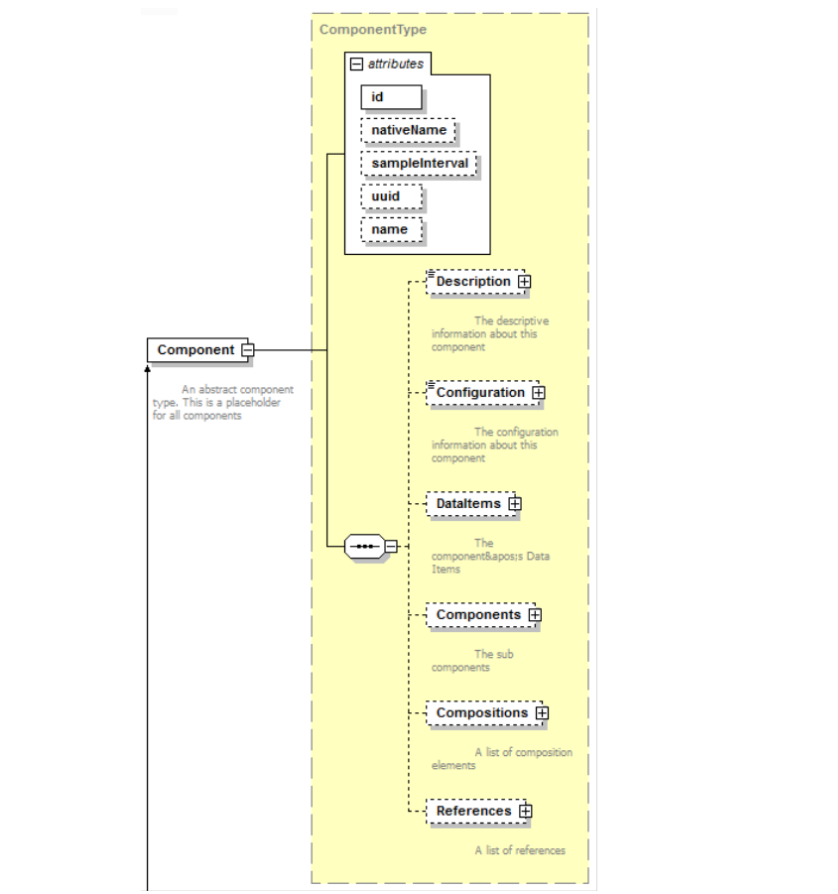
\includegraphics[width=1.0\textwidth]{figures/Components Schema.png}
  \caption{Components Schema Diagram}
  \label{fig:Components Schema Diagram}
\end{figure}

\FloatBarrier


\begin{figure}[ht]
  \centering
    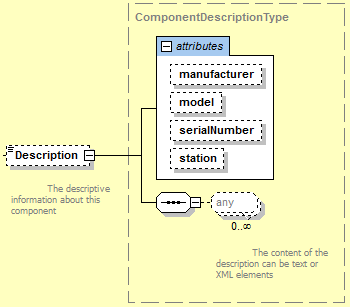
\includegraphics[width=1.0\textwidth]{figures/Component Description Schema.png}
  \caption{Component Description Schema Diagram}
  \label{fig:Component Description Schema Diagram}
\end{figure}

\FloatBarrier


\subsubsection{DataItems Schema Diagrams}
\label{sec:DataItems Schema Diagrams}

\begin{figure}[ht]
  \centering
    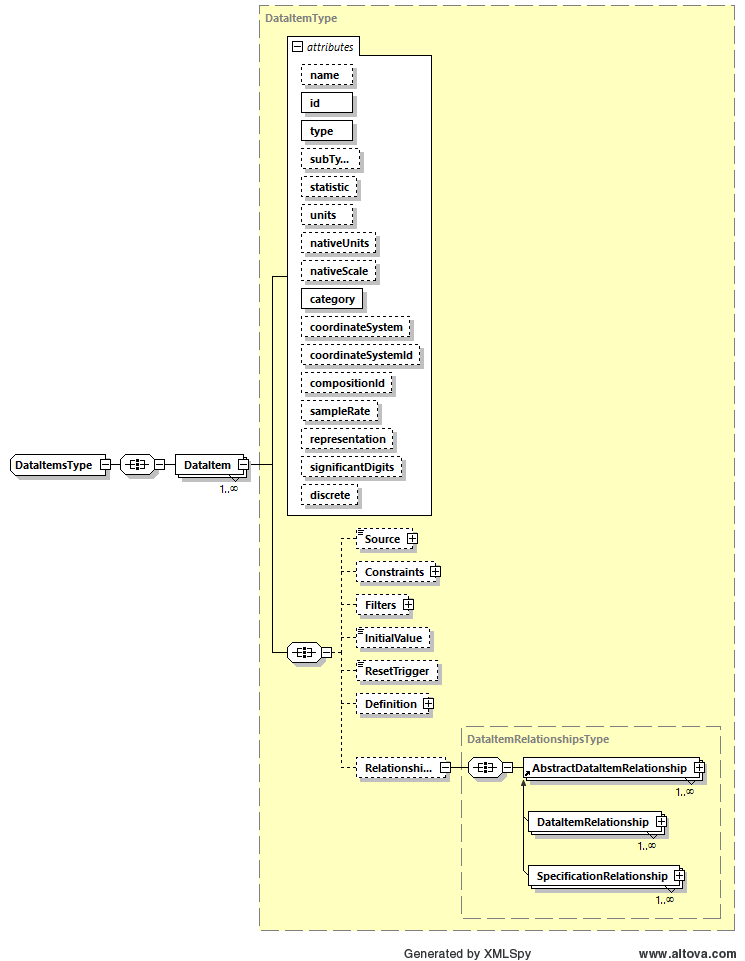
\includegraphics[width=1.0\textwidth]{figures/DataItems Schema.png}
  \caption{DataItems Schema Diagram}
  \label{fig:DataItems Schema Diagram}
\end{figure}

\FloatBarrier


\begin{figure}[ht]
  \centering
    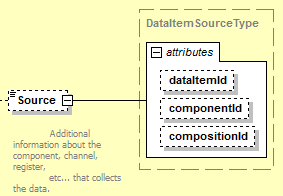
\includegraphics[width=1.0\textwidth]{figures/Source Schema.png}
  \caption{Source Schema Diagram}
  \label{fig:Source Schema Diagram}
\end{figure}

\FloatBarrier


\begin{figure}[ht]
  \centering
    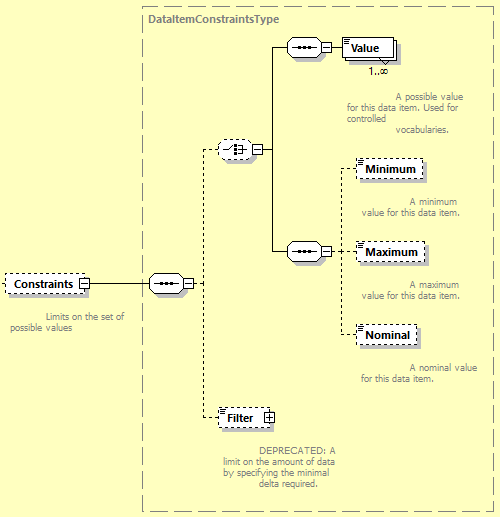
\includegraphics[width=1.0\textwidth]{figures/Constraints Schema.png}
  \caption{Constraints Schema Diagram}
  \label{fig:Constraints Schema Diagram}
\end{figure}

\FloatBarrier


\begin{figure}[ht]
  \centering
    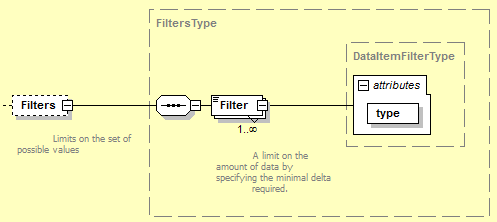
\includegraphics[width=1.0\textwidth]{figures/Filter Schema.png}
  \caption{Filter Schema Diagram}
  \label{fig:Filter Schema Diagram}
\end{figure}

\FloatBarrier


\begin{figure}[ht]
  \centering
    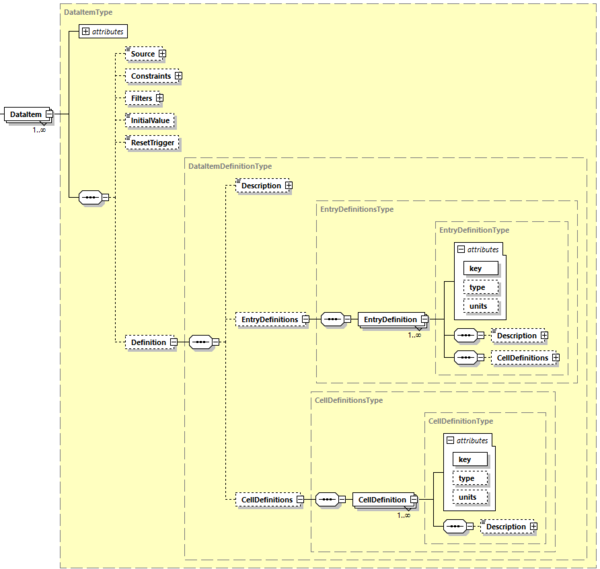
\includegraphics[width=1.0\textwidth]{figures/Definition Schema.png}
  \caption{Definition Schema Diagram}
  \label{fig:Definition Schema Diagram}
\end{figure}

\FloatBarrier


\subsubsection{References Schema Diagrams}
\label{sec:References Schema Diagrams}

\begin{figure}[ht]
  \centering
    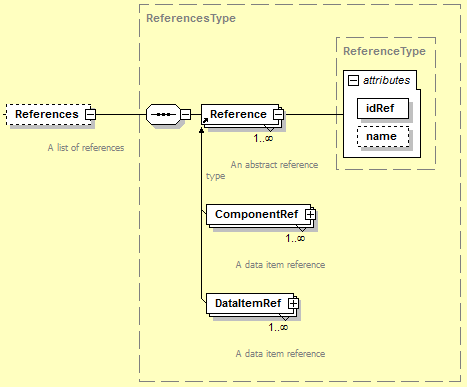
\includegraphics[width=1.0\textwidth]{figures/References Schema.png}
  \caption{References Schema Diagram}
  \label{fig:References Schema Diagram}
\end{figure}

\FloatBarrier


\begin{figure}[ht]
  \centering
    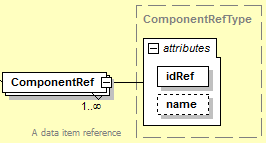
\includegraphics[width=1.0\textwidth]{figures/ComponentRef Schema.png}
  \caption{ComponentRef Schema Diagram}
  \label{fig:ComponentRef Schema Diagram}
\end{figure}

\FloatBarrier


\begin{figure}[ht]
  \centering
    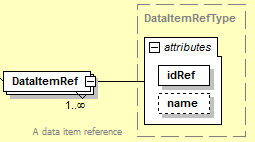
\includegraphics[width=1.0\textwidth]{figures/DataItemRef Schema.png}
  \caption{DataItemRef Schema Diagram}
  \label{fig:DataItemRef Schema Diagram}
\end{figure}

\FloatBarrier


\subsubsection{Configuration Schema Diagrams}
\label{sec:Configuration Schema Diagrams}

\begin{figure}[ht]
  \centering
    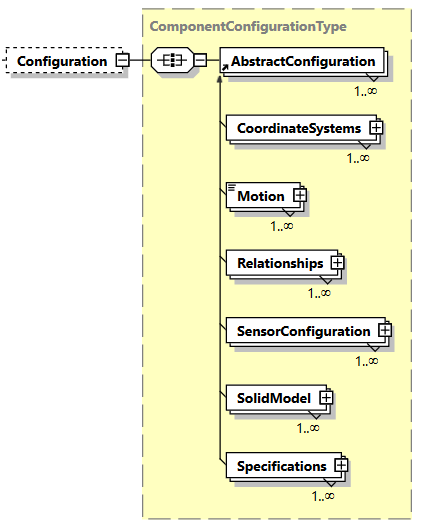
\includegraphics[width=1.0\textwidth]{figures/Configuration Schema.png}
  \caption{Configuration Schema Diagram}
  \label{fig:Configuration Schema Diagram}
\end{figure}

\FloatBarrier


\begin{figure}[ht]
  \centering
    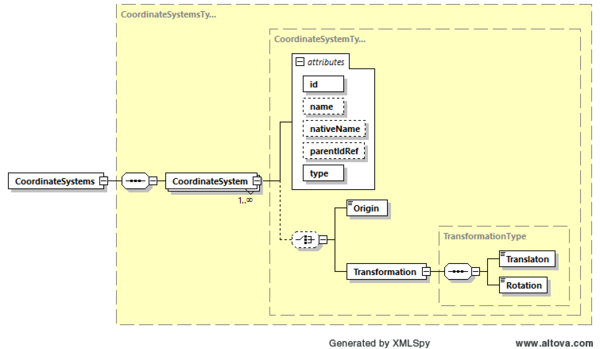
\includegraphics[width=1.0\textwidth]{figures/CoordinateSystem Schema.png}
  \caption{CoordinateSystem Schema Diagram}
  \label{fig:CoordinateSystem Schema Diagram}
\end{figure}

\FloatBarrier


\begin{figure}[ht]
  \centering
    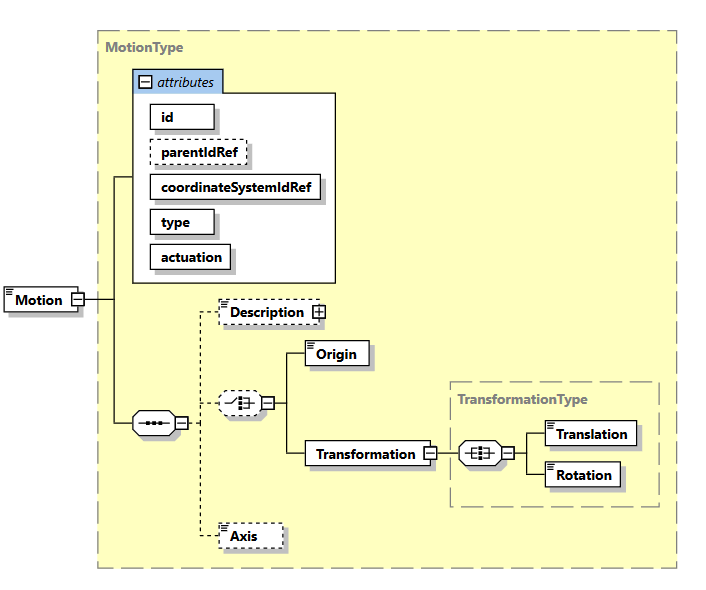
\includegraphics[width=1.0\textwidth]{figures/Motion Schema.png}
  \caption{Motion Schema Diagram}
  \label{fig:Motion Schema Diagram}
\end{figure}

\FloatBarrier


\begin{figure}[ht]
  \centering
    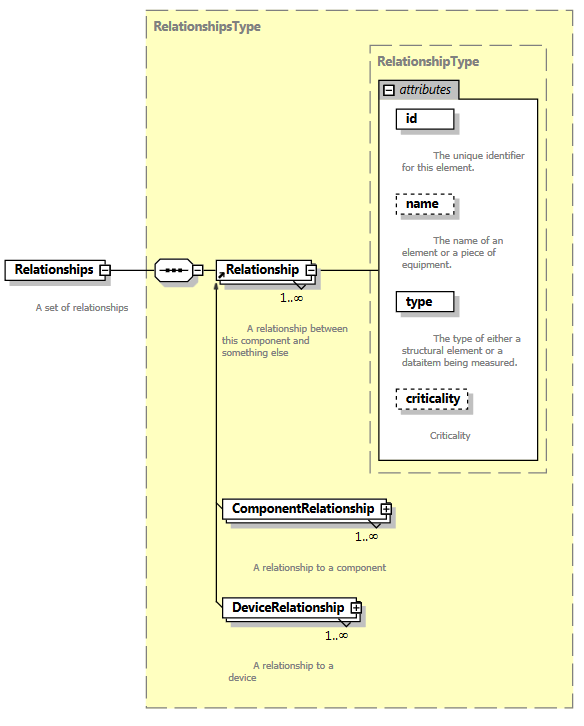
\includegraphics[width=1.0\textwidth]{figures/Relationships Schema.png}
  \caption{Relationships Schema Diagram}
  \label{fig:Relationships Schema Diagram}
\end{figure}

\FloatBarrier


\begin{figure}[ht]
  \centering
    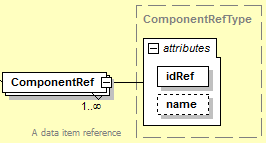
\includegraphics[width=1.0\textwidth]{figures/ComponentRelationship Schema.png}
  \caption{ComponentRelationship Schema Diagram}
  \label{fig:ComponentRelationship Schema Diagram}
\end{figure}

\FloatBarrier


\begin{figure}[ht]
  \centering
    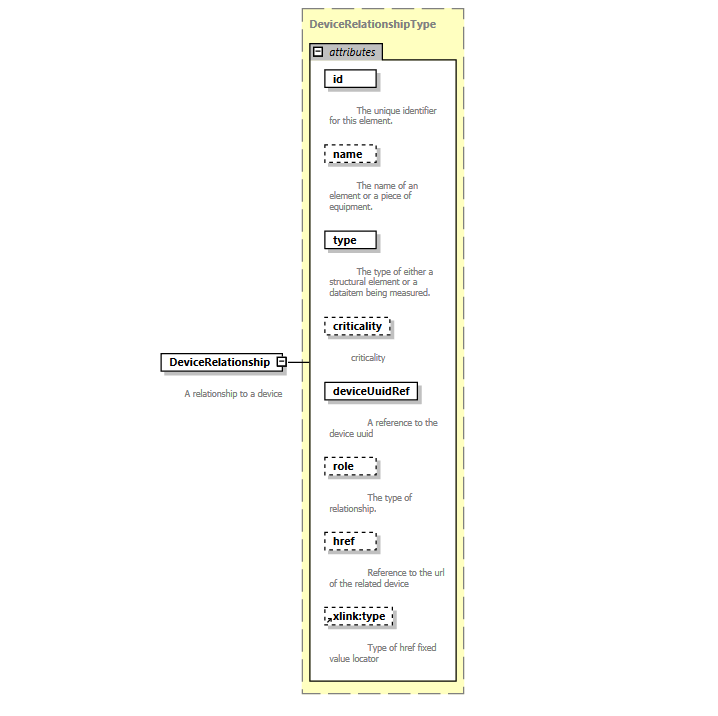
\includegraphics[width=1.0\textwidth]{figures/DeviceRelationship Schema.png}
  \caption{DeviceRelationship Schema Diagram}
  \label{fig:DeviceRelationship Schema Diagram}
\end{figure}

\FloatBarrier


\begin{figure}[ht]
  \centering
    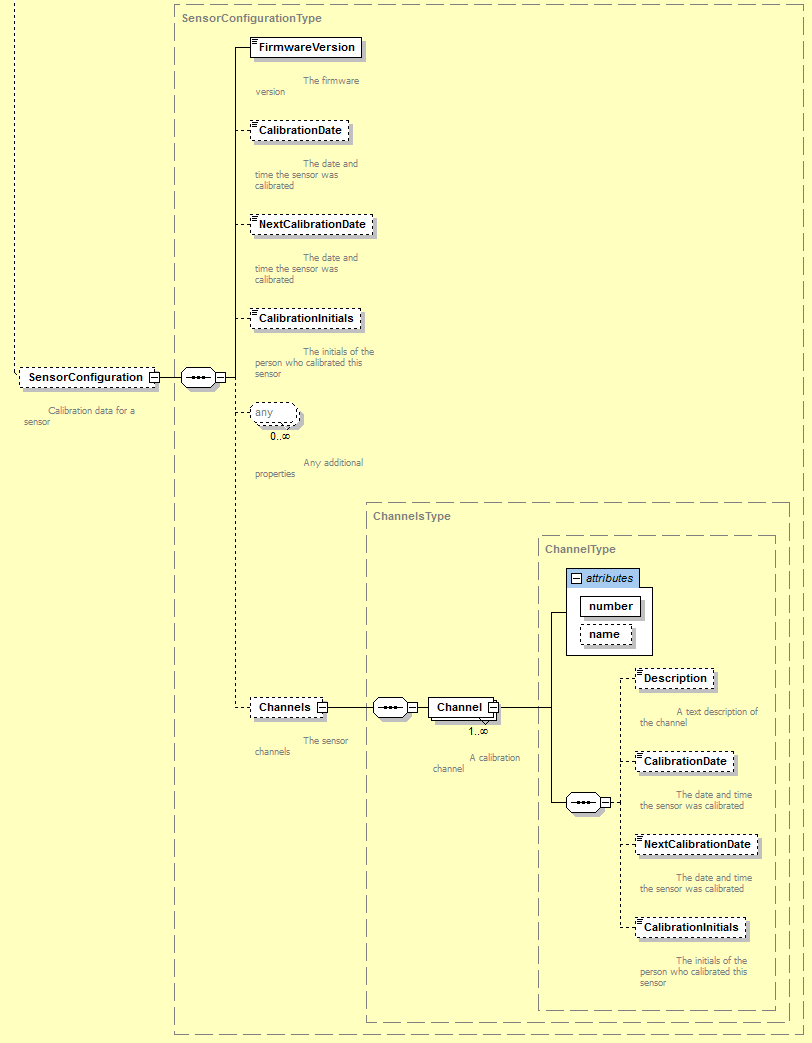
\includegraphics[width=1.0\textwidth]{figures/SensorConfiguration Schema.png}
  \caption{SensorConfiguration Schema Diagram}
  \label{fig:SensorConfiguration Schema Diagram}
\end{figure}

\FloatBarrier


\begin{figure}[ht]
  \centering
    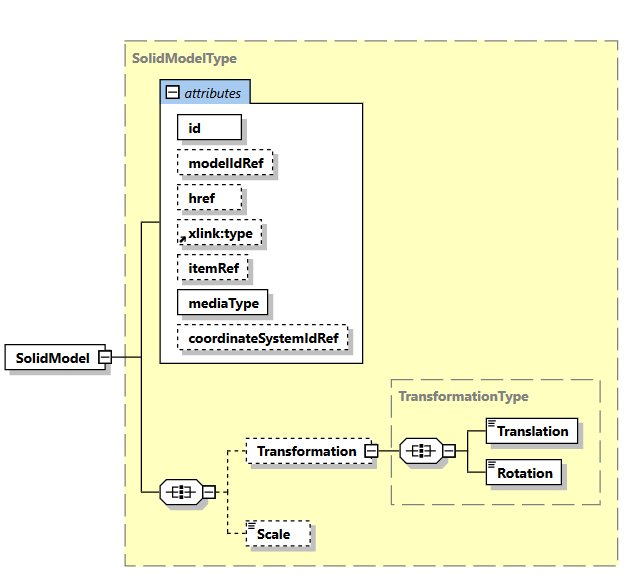
\includegraphics[width=1.0\textwidth]{figures/SolidModel Schema.png}
  \caption{SolidModel Schema Diagram}
  \label{fig:SolidModel Schema Diagram}
\end{figure}

\FloatBarrier


\begin{figure}[ht]
  \centering
    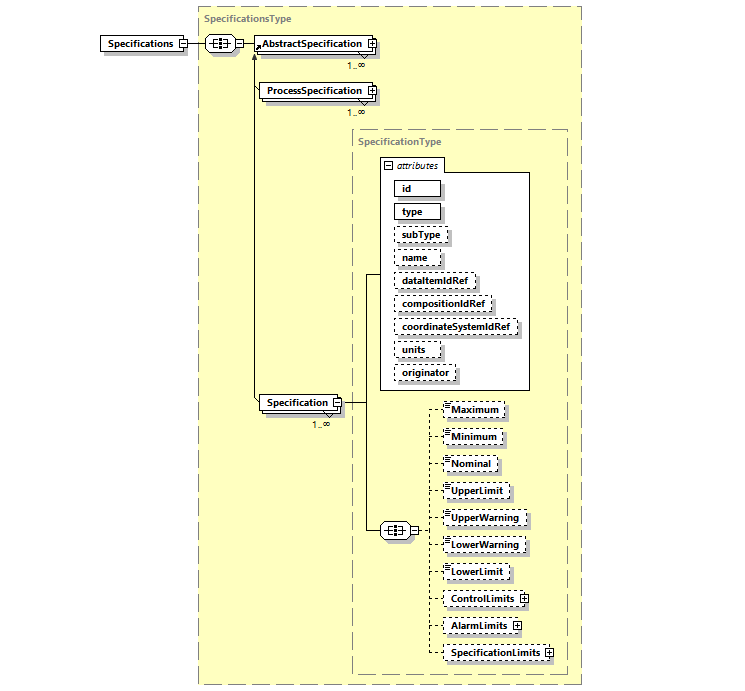
\includegraphics[width=1.0\textwidth]{figures/Specifications Schema.png}
  \caption{Specifications Schema Diagram}
  \label{fig:Specifications Schema Diagram}
\end{figure}

\FloatBarrier


\begin{figure}[ht]
  \centering
    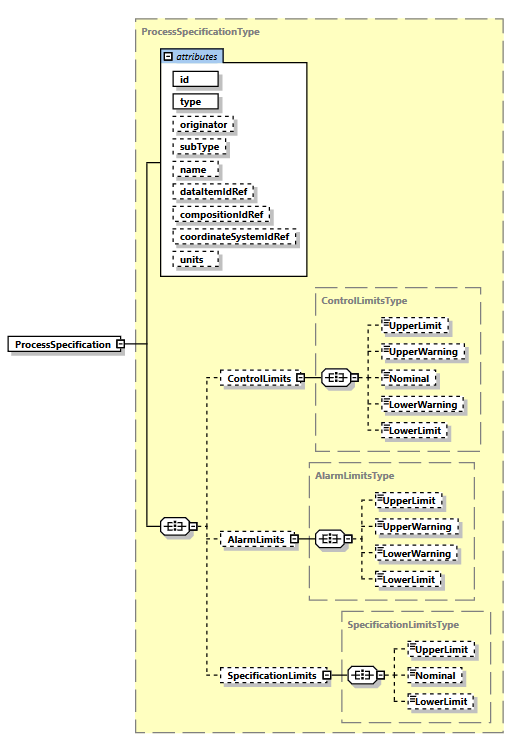
\includegraphics[width=1.0\textwidth]{figures/ProcessSpecification Schema.png}
  \caption{ProcessSpecification Schema Diagram}
  \label{fig:ProcessSpecification Schema Diagram}
\end{figure}

\FloatBarrier
